
\section{Limitaciones de la integración COMPSs+OmpSs-2}
\label{sec:estudiopreviorend}

En la sección \ref{sec:compssompss} se enunciaron los problemas que tuvimos con la integración inicial \textit{COMPSs+OmpSs}. En este apartado, se enuncian las limitaciones de la integración \textit{COMPSs+OmpSs-2}. En la anterior encontrábamos que las tareas de \textit{OmpSs} generadas dentro de una tarea de \textit{COMPSs} no tenían ningún tipo de aislamiento para el \textit{worker persistente}, y cuando se efectuaban esperas esto repercutía a absolutamente todas las tareas de \textit{OmpSs}. Utilizando el modo librería de \textit{OmpSs-2} proporcionamos a las tareas generadas dentro de una tarea de \textit{COMPSs} un ámbito propio, por lo cual las esperas tan sólo afectaran a las generadas dentro de esta, y no al resto.

\par\bigskip

Aún así, hemos encontrado limitaciones en la integración, para localizarlas hemos desarrollado una aplicación con dos tareas de diferente granularidad, con \textit{Extrae} y \textit{Paraver} veremos como se comporta la integración ante este caso. A grandes rasgos, la aplicación básicamente ejecuta 30 tareas de granularidad fina y gruesa, ésta se emula haciendo una espera bloqueante con \textit{usleep} de 50000 y 300000 microsegundos respectivamente. La implementación se encuentra en el apéndice \ref{appendix:estudioprevio}.

\par\bigskip

Cuándo el número de CPUs no es suficiente para la cantidad de tareas que \textit{OmpsS-2} crea, es propenso a la entremezcla.La planificación de las tareas no tiene por qué seguir ningún tipo de orden, la tarea que se ejecutará después no tiene por qué ser sucesora de esta o compartir predecesor, no hay ningún tipo de vínculo, se ejecuta lo que se cree mejor para explotar el paralelismo. Entonces una CPU que para nosotros tenía la expectativa de ejecutar tres tareas puede acabar ejecutando una mayor cantidad e incluso de una duración diferente. Este entremezclado puede derivar en una duración irregular de las tareas a nivel de \textit{COMPSs}, la siguiente imagen muestra una traza de \textit{COMPSs} y de \textit{OmpSs-2}.Entonces, si ejecutamos esta aplicación con un número de CPUs bajo y obtenemos una traza, veremos que las tareas se entremezclan, haciendo que una tarea que inicialmente debía tardar del orden de 50000 microsegundos acabe tardando 6 veces más. 

\begin{figure}[H]
	\centering 
	\caption{Duración irregular de las tareas de \textit{COMPSs}.}
	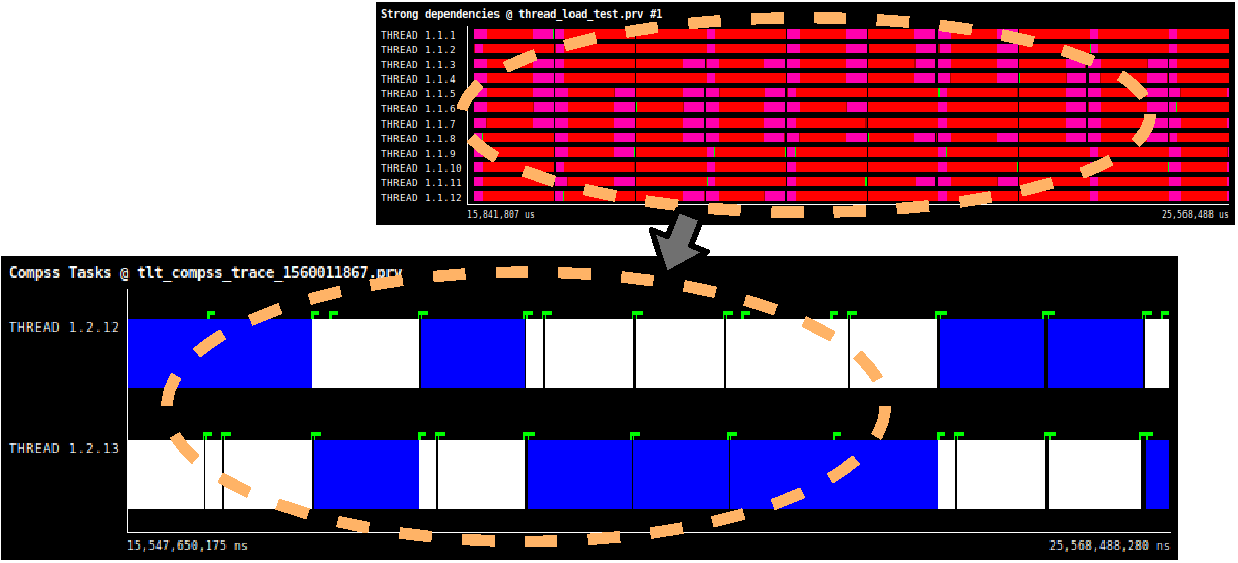
\includegraphics[scale=0.6]{estudio_previo/NERCOMPSsOmpSs.pdf}
	\label{fig:irregular}
\end{figure}

La imagen \ref{fig:irregular} muestra el comportamiento descrito, la traza superior corresponde a \textit{OmpSs-2}, es una parte de la aplicación, se puede apreciar el entremezclado de las tareas de granularidad fina y gruesa (rosa y rojo respectivamente), en la traza inferior de \textit{COMPSs} se observa que el entremezclado provoca que la duración de las tareas no sea uniforme, en algunos casos las de color blanco que son de granularidad fina tardan lo mismo o incluso más que las de color azul que son de granularidad gruesa. Recordemos que dentro de un mismo nodo, se comparte el \textit{runtime} de \textit{OmpSs-2} por lo cuál las tareas de \textit{COMPSs} que se ejecutan en un mismo nodo están sujetas a \textit{OmpSs-2} y no tienen entornos aislados entre sí. El hecho de que las tareas de \textit{COMPSs} tarden más o menos, es así por que \textit{OmpSs-2} constantemente ejecuta tareas en las CPUs que le parece mejor para explotar el paralelismo dentro del nodo, haciendo que una tarea de \textit{COMPSs} que podría ejecutar tan sólo lo que a ella le concierne ejecute también trabajo del resto, prolongando su duración (lo que vimos en la traza \ref{fig:irregular}).

\par\bigskip

Si aumentamos el número de CPUs, este comportamiento no debería repercutir de una manera tan drástica, con el aumento de recursos la duración de las tareas será más uniforme.

\begin{figure}[H]
	\centering 
	\caption{Duración regular de las tareas de \textit{COMPSs}.}
	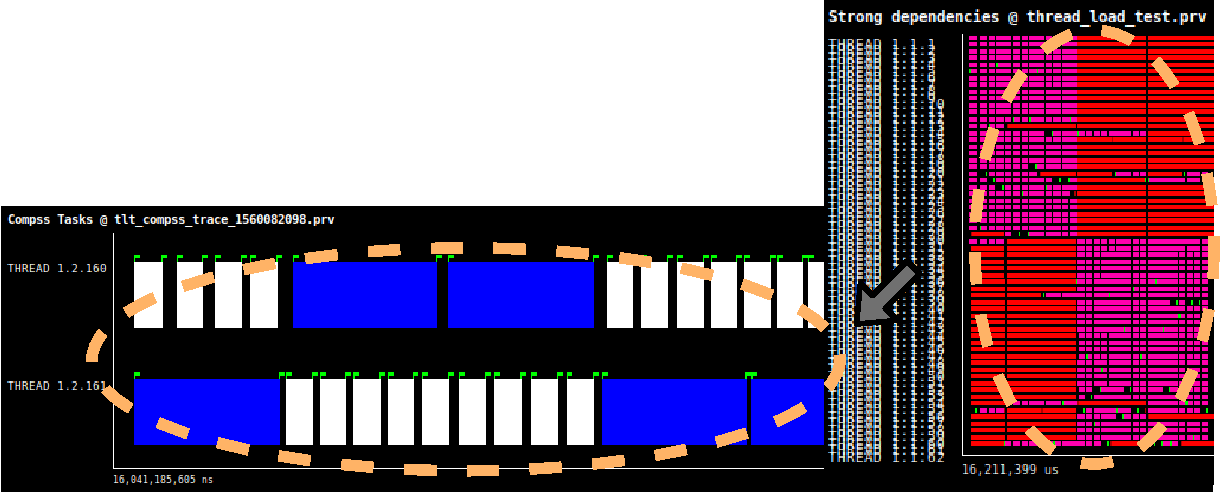
\includegraphics[scale=0.7]{estudio_previo/ERCOMPSsOmpSs.pdf}
	\label{fig:regular}
\end{figure}

En la ejecución de la imagen \ref{fig:regular} hay muchos más recursos, y como hemos anticipado esto hace que la duración de las tareas sea mucho más regular y por norma general no haya anomalías. Si la comparamos con la traza \ref{fig:irregular}, la duración de las tareas es mucho más regular, siempre son de la misma magnitud, y nunca una tarea de granularidad fina dura más que una gruesa. Esto se debe a que tenemos más recursos, por lo cuál no aparece el entremezclado de tareas y no se nos alargan las tareas de \textit{COMPSs}. Hay una diferenciación mucho más clara entre los dos tipos de tareas, y por lo general no existen estos conflictos por recursos que comentábamos. De todas formas, el comportamiento negativo que se ha enunciado con el primer par de trazas puede suceder eventualmente, ya que la manera en la que se gestionan los recursos no ha cambiado, pero mejora mucho.

\par\bigskip

Para eliminar esta limitación, habría que otorgar a cada tarea generada a través de la función \textit{nanos6\_spawn\_function} un subconjunto de los recursos o organizar la planificación con prioridades descendientes entre tareas consecutivas generadas vía \textit{spawn}, con la primera opción las tareas de \textit{OmpSs-2} generadas en una tarea de \textit{COMPSs} no harían ni sufrirían interferencias ya que tienen recursos propios asignados, y con la segunda opción se ejecutarían en orden, por lo que tampoco habría interferencias con ni sobre el resto.

